\section{Estudio experimental}

Este capítulo describe el diseño y los resultados de un experimento computacional realizado para evaluar el rendimiento de los algoritmos presentados en el capítulo anterior. El objetivo principal es comparar la eficacia de los algoritmos genéticos con y sin las mejoras propuestas, en términos de calidad de las soluciones y tiempo de ejecución. Para ello, se generaron instancias de prueba aleatorias. Los resultados se analizan y discuten en el contexto del problema de llenado de contenedores.

\subsection{Generación de datos de prueba}

En la literatura, se han propuesto diversos conjuntos de instancias de prueba para evaluar algoritmos de llenado de contenedores. Por ejemplo, \textcite{BISCHOFF1995377} establecieron un método de generación de instancias que se ha utilizado ampliamente en estudios posteriores. Sin embargo, debido a las restricciones del llenado manual, las instancias públicas no son adecuadas para experimentos computacionales. Esto se debe a que, al usar el procedimiento manual descrito en la sección \ref{sec:problem}, las soluciones son menos óptimas en comparación con los algoritmos que no consideran estas restricciones. Por tanto, se decidió generar instancias aleatorias siguiendo un enfoque más realista.

Las siguientes restricciones se consideraron para generar las instancias de prueba:

\begin{itemize}
    \item Las unidades de medida son milímetros, redondeadas al entero más cercano.
    \item El contenedor tiene dimensiones interiores fijas: $L \times W \times H = 12010 \times 2330 \times 2380$ mm.
    \item Cada instancia incluye un número fijo de tipos de cajas: 5, 10, 20, 30, 40, 50, denominadas 5T, 10T, 20T, 30T, 40T y 50T, respectivamente.
    \item Las cajas de tipo 5T están contenidas en las de tipo 10T, las de 10T en las de 20T y asi sucesivamente.
    \item Las dimensiones de las cajas se generan aleatoriamente siguiendo una distribución uniforme en el rango $[250, 750]$ mm.
    \item Los valores de las cajas se generan aleatoriamente siguiendo una distribución uniforme en el rango $[1, 100]$, dependiendo del tamaño.
\end{itemize}

Para aumentar la diversidad, se asegura que las dimensiones de las cajas no se repitan dentro de cada instancia. El Algoritmo \ref{alg:evitar_repetir} detalla el procedimiento para evitar la repetición de dimensiones.

\begin{algorithm}[H]
    \caption{Evitar repetir dimensiones}
    \label{alg:evitar_repetir}
    \begin{algorithmic}[1]
        \Require $|T|$, cantidad de cajas a generar.
        \Require $RangoDimensiones$, rango de dimensiones.
        \Ensure $D$, lista de dimensiones.
        \State $D \gets \emptyset$
        \For{$i \gets 1$ \textbf{to} $|T|$}
        \State $d \gets \text{Aleatorio}(RangoDimensiones)$
        \While{$d \in D$}
        \State $d \gets \text{Aleatorio}(RangoDimensiones)$
        \EndWhile
        \State $D \gets D \cup d$
        \EndFor
        \State \textbf{return} $D$
    \end{algorithmic}
\end{algorithm}

En el Algoritmo \ref{alg:evitar_repetir}, $|T|$ es la cantidad de cajas a generar. En la línea 1, se inicializa la lista $D$ de dimensiones. En las líneas 2 a 8, se itera sobre la cantidad de cajas a generar. En la línea 3, se genera una dimensión aleatoria y en la línea 4, se verifica si la dimensión ya existe en la lista $D$. Si es así, se vuelve a generar una dimensión aleatoria (línea 5) hasta que se obtenga una dimensión única. Finalmente, en la línea 9, se retorna la lista $D$ con las dimensiones generadas.

Para determinar la cantidad máxima de cajas de cada tipo que se puede almacenar en un contenedor, se sigue el siguiente enfoque:

1. Dividir el volumen total del contenedor por el número de tipos de cajas especificados. Por ejemplo, cinco tipos de cajas resultan en dividir el contenedor en cinco partes iguales ("5T").
2. Calcular cuántas cajas de cada tipo caben exactamente en la fracción del volumen asignada a ese tipo.
3. Añadir un porcentaje aleatorio de cajas adicionales a cada tipo para aumentar el desafío y realismo.

Este procedimiento se detalla en el Algoritmo \ref{alg:generate}.

\begin{algorithm}[H]
    \caption{Generación de cantidades de cajas}
    \label{alg:generate}
    \begin{algorithmic}[1]
        \Require $V_{\text{total}}$, volumen total del contenedor; $T$, tipos de cajas.
        \Ensure $Q$, lista de cantidades por tipo.
        \State $Q \gets \emptyset$
        \State $v_{\text{fraccion}} \gets V_{\text{total}} / |T|$ \Comment{Dividir el volumen total en partes iguales}
        \For{$t_i \in T$}
        \State $v_i \gets w_i \times l_i \times h_i$ \Comment{Volumen de un tipo $t_i$}
        \State $q_i \gets \lceil v_{\text{fraccion}} / v_i \rceil$
        \State $q_i^{\text{ajustado}} \gets q_i + \text{Aleatorio}(\% \text{adicional})$ \Comment{Añadir un porcentaje aleatorio}
        \State $Q \gets Q \cup q_i^{\text{ajustado}}$
        \EndFor
        \State \textbf{return} $Q$
    \end{algorithmic}
\end{algorithm}

En el Algoritmo \ref{alg:generate}, $V_{\text{total}}$ es el volumen total del contenedor, y $T$ es el conjunto de tipos de cajas. Primero, se inicializa la lista $Q$ de cantidades por tipo (línea 1). Luego, se calcula la fracción del volumen total asignada a cada tipo de caja (línea 2). En las líneas 3 a 8, se calcula el volumen de cada tipo de caja, la cantidad aproximada de cajas que caben en la fracción del volumen asignada y se ajusta esta cantidad añadiendo un porcentaje aleatorio. Finalmente, se retorna la lista $Q$ con las cantidades ajustadas por tipo (línea 9).

El procedimiento completo para generar las instancias de prueba es:

\begin{enumerate}
    \item Generar un conjunto de dimensiones únicas de cajas para cada tipo de caja según el Algoritmo \ref{alg:evitar_repetir}.
    \item Asignar un valor aleatorio a cada caja.
    \item Generar un conjunto de cantidades de cajas para cada tipo de caja, según el Algoritmo \ref{alg:generate}.
\end{enumerate}

Este procedimiento se resume en el Algoritmo \ref{alg:generate_instances}.

\begin{algorithm}[H]
    \caption{Generación de instancias de prueba}
    \label{alg:generate_instances}
    \begin{algorithmic}[1]
        \Require $V_{\text{total}}$, volumen total del contenedor; $C$, cantidad de problemas por tipo; $T$, tipos de cajas.
        \Ensure $P$, lista de instancias de problemas.
        \State $P \gets \emptyset$
        \For{$t_i \in T$}
        \For{$c \gets 1$ \textbf{to} $C$}
        \State $D \gets \text{EvitarRepetirDimensiones}(|T|, RangoDimensiones)$
        \State $V \gets \text{Aleatorio}(|T|, RangoValores)$
        \State $Q \gets \text{GenerarCantidades}(V_{\text{total}}, T)$
        \State $P \gets P \cup (D, V, Q)$
        \EndFor
        \EndFor
        \State \textbf{return} $P$
    \end{algorithmic}
\end{algorithm}

En el Algoritmo \ref{alg:generate_instances}, $V_{\text{total}}$ es el volumen total del contenedor, $C$ es la cantidad de problemas por tipo de caja, y $T$ es el conjunto de tipos de cajas. Primero, se inicializa la lista vacía $P$ de instancias de problemas (línea 1). Luego, se itera sobre la cantidad de tipos de cajas y la cantidad de problemas por tipo de caja. Para cada iteración, se genera un conjunto de dimensiones únicas de cajas, se asignan valores aleatorios y se genera un conjunto de cantidades de cajas para cada tipo de caja. Finalmente, se retorna la lista $P$ con las instancias de problemas generadas (línea 9). Por ejemplo, si hay 4 tipos de cajas (5T, 10T, 20T, 30T) y se desean generar 10 problemas por tipo, se obtendrán 40 instancias de problemas en total.

\subsection{Diseño del experimento}

Para evaluar el rendimiento de los algoritmos genéticos propuestos, se diseñó un experimento computacional que compara los resultados obtenidos con y sin las mejoras propuestas. Se considera una versión sin mejora llamada M0 y cuatro mejoras denominadas M1, M2, M3 y M4, descritas a continuación:

\begin{itemize}
    \item M0: Versión sin mejoras del algoritmo genético.
    \item M1: Mejora de \textit{llenado adicional inmediato}, completando espacios restantes durante el proceso de llenado (Algoritmo \ref{alg:dblf_adaptado_mejoras_m1}).
    \item M2: Mejora de \textit{llenado adicional al final}, completando los espacios restantes al final del proceso de llenado en toda la población (Algoritmo \ref{alg:dblf_adaptado_mejoras_m2}).
    \item M3: Extensión de M2, aplicada a la mitad superior de los individuos según su desempeño.
    \item M4: Mejora de M2, aplicada exclusivamente al mejor individuo de la población.
\end{itemize}

Los algoritmos se implementaron en Python v3.10 y están disponibles en un repositorio de GitHub\footnote{\url{https://github.com/josegustavo/lcp}}.

El experimento se ejecutó en un equipo con un procesador Apple M1 de 8 núcleos (4 núcleos de eficiencia y 4 de rendimiento) y 8 GB de RAM. Para optimizar el uso de los recursos, se paralelizó la ejecución de los algoritmos genéticos para utilizar los 4 núcleos de rendimiento, y se empleó la librería Pypy como intérprete de Python.

Se crearon 25 instancias para cada tipo de caja (5T, 10T, 20T, 30T, 40T y 50T), sumando un total de 150 instancias de prueba. Cada instancia se ejecutó con las mejoras propuestas M0, M1, M2, M3 y M4 para comparar los resultados.

Cada algoritmo genético se configuró con una población inicial de 100 individuos y un tiempo de ejecución límite de 5 minutos, asegurando condiciones uniformes para la evaluación comparativa. La probabilidad de cruce ($P_{CROSS}$) se estableció en 0.05 y la probabilidad de mutación ($P_{MUT}$) en 0.01. Estos valores fueron seleccionados después de experimentaciones previas que demostraron su eficacia al promover un equilibrio adecuado entre exploración y explotación durante el proceso evolutivo.

Los resultados fueron almacenados en archivos CSV para su posterior análisis. Se evaluaron dos métricas principales: el valor aportado por las soluciones obtenidas y el tiempo de ejecución. También se inspeccionaron aleatoriamente algunas soluciones generadas para verificar su validez y coherencia con las restricciones del problema. Se utilizó la librería Matplotlib para visualizar los resultados y verificar visualmente la calidad de las soluciones obtenidas. Por ejemplo en la Figura \ref{fig:ejemplo_solucion}, se muestra una solución óptima encontrada por el algoritmo genético.

\begin{figure}[H]
    \centering
    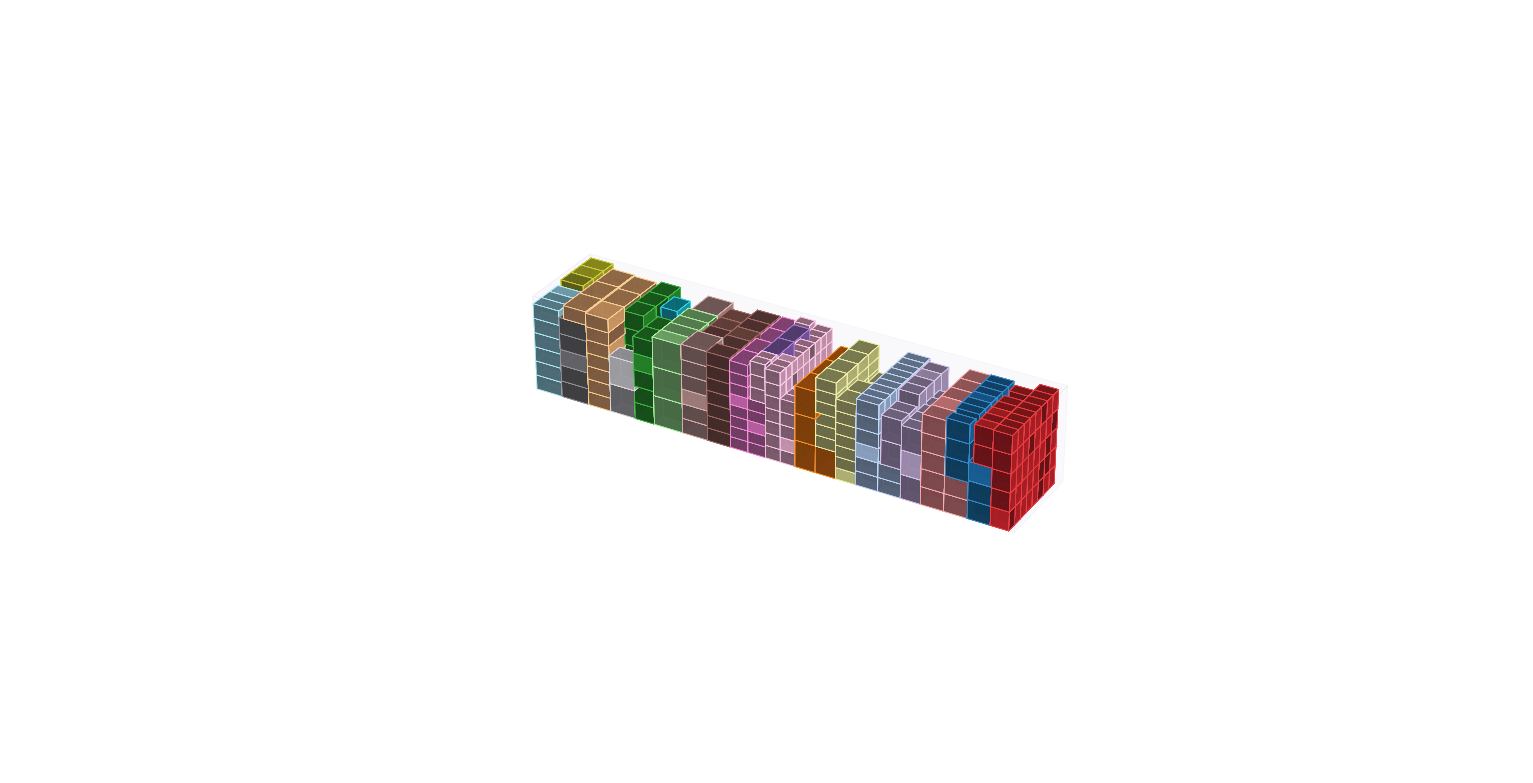
\includegraphics[width=0.8\textwidth]{Figures/ejemplo_solucion.eps}
    \caption{Ejemplo de una solución final generada por el algoritmo genético}
    \label{fig:ejemplo_solucion}
\end{figure}

\subsection{Resultados y análisis}

En esta sección se presentan y analizan los resultados obtenidos del experimento computacional. Los resultados se agrupan en función de las mejoras implementadas (M0, M1, M2, M3 y M4) y el tipo de instancia (5T, 10T, 20T, 30T, 40T, 50T). Se evalúan dos métricas principales: el valor aportado por las soluciones obtenidas y el tiempo de ejecución.

El valor aportado por las soluciones indica qué tan bueno es el resultado final obtenido en comparación con la población inicial. Por otro lado, el tiempo de ejecución mide cuánto tiempo tarda el algoritmo en encontrar la mejor solución. También a partir de estas métricas se calcula el rendimiento de las mejoras propuestas, que indica el incremento porcentual en la calidad de las soluciones por cada unidad de tiempo. Con estos resultados, se evalúa la eficacia de las mejoras propuestas.

\subsubsection{Valor aportado por las soluciones}

Dado que los valores de las cajas en las diferentes instancias son aleatorios, no es posible comparar directamente los valores totales de las soluciones obtenidas. Por ello, se utiliza una métrica relativa que indica el porcentaje de mejora desde la población inicial. Se toma el mejor valor obtenido al final y se calcula el incremento en porcentaje tomando como base el mejor valor de la población inicial, que al ser común para todas las estrategias de mejora, permite una comparación justa.

El porcentaje de mejora se calcula por tipo de caja y mejora propuesta. Los resultados promediados sobre las 25 instancias se muestran en la Tabla \ref{tab:valor_aportado}, presentando el promedio y la desviación estándar para cada mejora.

\begin{table}[H]
    \centering
    \caption{Valor aportado por las soluciones obtenidas}
    \label{tab:valor_aportado}
    \begin{tabular}{|c|c|c|c|c|c|c|c|c|c|c|}
        \hline
        \multirow{2}{*}{\textbf{Tipo de Caja}} & \multicolumn{2}{c|}{\textbf{M0}} & \multicolumn{2}{c|}{\textbf{M1}} & \multicolumn{2}{c|}{\textbf{M2}} & \multicolumn{2}{c|}{\textbf{M3}} & \multicolumn{2}{c|}{\textbf{M4}}                                                                             \\ \cline{2-11}
                                               & \textbf{media}                   & \textbf{sd}                      & \textbf{media}                   & \textbf{sd}                      & \textbf{media}                   & \textbf{sd} & \textbf{media} & \textbf{sd} & \textbf{media} & \textbf{sd} \\ \hline
        5T                                     & 9.3\%                            & 3.7                              & 10.5\%                           & 4.1                              & 10.4\%                           & 4.1         & 10.0\%         & 4.1         & 9.9\%          & 4.1         \\ \hline
        10T                                    & 18.5\%                           & 6.0                              & 20.9\%                           & 6.1                              & 20.6\%                           & 5.9         & 20.2\%         & 6.1         & 19.0\%         & 5.9         \\ \hline
        20T                                    & 27.2\%                           & 6.5                              & 33.1\%                           & 6.6                              & 32.1\%                           & 6.5         & 31.6\%         & 6.6         & 28.3\%         & 7.0         \\ \hline
        30T                                    & 29.0\%                           & 7.8                              & 37.8\%                           & 8.7                              & 37.2\%                           & 8.9         & 34.9\%         & 7.9         & 31.8\%         & 8.1         \\ \hline
        40T                                    & 28.6\%                           & 8.3                              & 44.5\%                           & 9.8                              & 43.1\%                           & 10.1        & 42.2\%         & 9.8         & 35.1\%         & 9.7         \\ \hline
        50T                                    & 35.2\%                           & 9.4                              & 56.7\%                           & 12.6                             & 54.6\%                           & 12.5        & 52.1\%         & 13.2        & 46.4\%         & 12.3        \\ \hline
    \end{tabular}
\end{table}

Como se observa en la Tabla \ref{tab:valor_aportado}, todas las mejoras propuestas (M1, M2, M3 y M4) superan a la versión sin mejoras (M0) en términos de valor aportado por las soluciones obtenidas. Las mejoras M1 y M2, que se aplican a toda la población, muestran los mejores resultados en todos los casos, aumentando la calidad de las soluciones en comparación con las demás versiones de mejora. También se observa que el valor aportado por las soluciones aumenta a medida que se incrementa el número de tipos de cajas a llenar, esto debido a que mientras mayor sean los tipos de cajas, el problema se vuelve más complejo y las soluciones iniciales tienden a ser peores lo que permite que las mejoras tengan un mayor impacto. Esto se puede observar en la Figura \ref{fig:valores}.

\begin{figure}[H]
    \centering
    \includesvg[width=0.8\textwidth]{Figures/improvement.svg}
    \caption{Valor aportado por las soluciones obtenidas}
    \label{fig:valores}
\end{figure}


La Figura \ref{fig:valores} muestra el valor en porcentaje aportado por las soluciones obtenidas para cada mejora (M0, M1, M2, M3, M4) y tipo de instancia (5T, 10T, 20T, 30T, 40T, 50T). Se observa que las mejoras M1 y M2 presentan un mayor valor aportado por las soluciones en comparación con M0, M3 y M4. Por otro lado, se destaca que cuando la complejidad del problema no es muy alta (5T y 10T), todas las mejoras presentan desempeños similares, pero a medida que la complejidad aumenta, se observa una clara diferencia entre las mejoras.


\subsubsection{Tiempo de ejecución}

El tiempo de ejecución es una métrica crucial para evaluar la eficiencia de los algoritmos genéticos, debido a que no se puede prever cuánto tiempo tomará encontrar la mejor solución. En este experimento, se midió el tiempo de ejecución de cada mejora y tipo de instancia, con el objetivo de evaluar el impacto de las mejoras en el tiempo de ejecución de los algoritmos.

Se propusieron las mejoras M3 y M4 con la expectativa de reducir el tiempo de ejecución en comparación con M2, sin comprometer la calidad de las soluciones. M3 aplica la mejora al final del llenado M2, pero solo a la mitad de la población, mientras que M4 la aplica solo al mejor individuo. Es crucial evaluar si estas mejoras efectivamente logran su objetivo de reducir el tiempo de ejecución y si mantienen la calidad de las soluciones obtenidas.

Cada ejecución se realiza con un conjunto de tipos de cajas y una implementación específica (M0, M1, M2, M3 y M4). Como se estableció un límite de tiempo de 5 minutos para cada ejecución, se registra el tiempo que cada evaluación tarda en encontrar su mejor solución.

En la Tabla \ref{tab:tiempo}, se muestra el tiempo promedio en encontrar la mejor solución (en segundos), junto a la desviación estándar, para cada mejora y tipo de instancia.

\begin{table}[H]
    \centering
    \caption{Tiempo promedio en encontrar la mejor solución}
    \label{tab:tiempo}
    \begin{tabular}{|c|c|c|c|c|c|c|c|c|c|c|}
        \hline
        \multirow{2}{*}{\textbf{Tipo de Caja}} & \multicolumn{2}{c|}{\textbf{M0}} & \multicolumn{2}{c|}{\textbf{M1}} & \multicolumn{2}{c|}{\textbf{M2}} & \multicolumn{2}{c|}{\textbf{M3}} & \multicolumn{2}{c|}{\textbf{M4}}                                                                             \\ \cline{2-11}
                                               & \textbf{media}                   & \textbf{sd}                      & \textbf{media}                   & \textbf{sd}                      & \textbf{media}                   & \textbf{sd} & \textbf{media} & \textbf{sd} & \textbf{media} & \textbf{sd} \\ \hline
        5T                                     & 71.4                             & 72.4                             & 23.7                             & 47.6                             & 56.9                             & 71.1        & 33.6           & 63.5        & 39.3           & 47.9        \\ \hline
        10T                                    & 146.0                            & 85.3                             & 72.5                             & 69.2                             & 102.1                            & 87.9        & 61.1           & 59.8        & 117.5          & 85.8        \\ \hline
        20T                                    & 214.4                            & 56.4                             & 89.0                             & 72.6                             & 145.9                            & 62.6        & 188.0          & 79.7        & 166.8          & 70.8        \\ \hline
        30T                                    & 263.1                            & 36.3                             & 183.8                            & 73.9                             & 175.4                            & 81.9        & 186.8          & 70.4        & 231.9          & 48.9        \\ \hline
        40T                                    & 266.2                            & 34.0                             & 208.4                            & 70.0                             & 224.0                            & 50.9        & 244.0          & 49.1        & 238.3          & 54.2        \\ \hline
        50T                                    & 257.0                            & 42.6                             & 244.3                            & 49.2                             & 228.5                            & 61.3        & 251.7          & 36.4        & 250.5          & 51.6        \\ \hline
    \end{tabular}
\end{table}

La Tabla \ref{tab:tiempo} muestra que las mejoras introducidas (M1, M2, M3 y M4), a pesar de que requieren tiempo adicional para realizar las operaciones de mejora, reducen ligeramente el tiempo necesario para encontrar la mejor solución en comparación con M0. Esto se debe a que las mejoras permiten que el algoritmo genético converja más rápidamente. Sin embargo, también se observa una tendencia al aumento del tiempo de convergencia a medida que se incrementa el número de tipos de cajas a llenar, lo que se debe a la mayor complejidad del problema. Incluso los valores cercanos a 300 segundos (5 minutos) podría indicar que el algoritmo aún no puede encontrar la mejor solución en el tiempo límite establecido. Esto se puede observar en la Figura \ref{fig:tiempos}.

\begin{figure}[H]
    \centering
    \includesvg[width=0.8\textwidth]{Figures/tiempos.svg}
    \caption{Tiempo promedio en encontrar la mejor solución}
    \label{fig:tiempos}
\end{figure}

La Figura \ref{fig:tiempos} destaca que la mejora M1 presenta el menor tiempo de convergencia en comparación con los otros casos, seguida de M2 y M3 en algunas situaciones. La versión sin mejoras, M0, muestra un tiempo de convergencia significativamente mayor en comparación con las versiones mejoradas. Esto confirma que las mejoras propuestas permiten que el algoritmo genético converja más rápidamente.

También se puede evaluar el tiempo que cada método de mejora necesita para evaluar una generación en una población de 100 individuos. Esto se calcula dividiendo el tiempo total de ejecución, que es de 300 segundos fijos para todos los métodos, por la cantidad de generaciones realizadas. Así obtenemos una idea del tiempo que cada método de mejora requiere para evaluar una generación. En la Figura \ref{fig:tiempo_generacion}, se muestra el tiempo promedio en milisegundos que toma cada método de mejora para evaluar una generación.

\begin{figure}[H]
    \centering
    \includesvg[width=0.8\textwidth]{Figures/tiempo_generacion.svg}
    \caption{Tiempo promedio en evaluar una población}
    \label{fig:tiempo_generacion}
\end{figure}

La Figura \ref{fig:tiempo_generacion} confirma que las mejoras M1, M2, M3 y M4 necesitan más tiempo para evaluar una generación en comparación con la versión sin mejoras M0. Esto se debe a que las mejoras requieren tiempo adicional para ejecutar las algoritmos de mejora propuestos. Sin embargo, como se ha mostrado en los gráficos anteriores, las mejoras también permiten que el algoritmo genético converja más rápidamente, lo que compensa el tiempo adicional requerido para realizar las operaciones de mejora.

\subsubsection{Rendimiento}

Para proporcionar una visión clara del impacto de las mejoras, se presenta un análisis comparativo del rendimiento, definido como el \textbf{incremento porcentual en la calidad de las soluciones por cada unidad de tiempo}. La Figura \ref{fig:rendimiento} muestra el rendimiento de las mejoras propuestas en términos de calidad de las soluciones y tiempo de ejecución.

\begin{figure}[H]
    \centering
    \includesvg[width=0.8\textwidth]{Figures/rendimiento.svg}
    \caption{Rendimiento de las mejoras propuestas}
    \label{fig:rendimiento}
\end{figure}

Las líneas de la Figura \ref{fig:rendimiento} se pueden interpretar como cuanto valor en porcentaje se gana por cada segundo de tiempo de ejecución. Se observa que la mejora M1 proporciona el mayor incremento porcentual en la calidad de las soluciones por cada segundo, seguida de M2 y M3 en algunas situaciones. La versión sin mejoras, M0, muestra un rendimiento significativamente menor en comparación con las versiones mejoradas.

\subsection{Evaluando el progreso de las soluciones}

Para evaluar el progreso de las soluciones a lo largo de las generaciones, se analiza el valor aportado por las soluciones obtenidas durante todo el tiempo de ejecución. Este análisis se centra exclusivamente en la mejora M1, dado que presenta el mejor rendimiento en términos de calidad de las soluciones y tiempo de convergencia. Además, se incluye en el gráfico la versión sin mejoras (M0) para mostrar la diferencia en ambos casos. Además para simplificar el análisis, se considera solo algunas instancias representativas (10T, 30T, 50T).

En la Figura \ref{fig:progreso}, se muestra el progreso de las soluciones obtenidas por M0 y M1 en las instancias de prueba con 10, 30 y 50 tipos de cajas (10T, 30T, 50T).

\begin{figure}[H]
    \centering
    \includesvg[width=0.8\textwidth]{Figures/progreso.svg}
    \caption{Progreso de las soluciones obtenidas por M0 y M1 para 10T, 30T, 50T}
    \label{fig:progreso}
\end{figure}

La Figura \ref{fig:progreso} muestra que M1 logra superar a M0 en términos de calidad de las soluciones en todas las instancias de prueba. Además, se observa que M1 converge más rápidamente a soluciones de alta calidad en comparación con M0. Por otro lado, M0 muestra un progreso más lento en comparación con M1. Esto confirma que la mejora M1 permite que el algoritmo genético converja más rápidamente y obtenga soluciones de mayor calidad en comparación con la versión sin mejoras. También es importante destacar que a medida que se incrementa el número de tipos de cajas a llenar, la convergencia se pierde, lo que indica que posiblemente en esos casos el algoritmo necesita más tiempo para encontrar la mejor solución.

Por último, es importante resaltar que la mejora M1 es la que muestra mejor rendimiento en términos de calidad de las soluciones y tiempo de convergencia en la mayoría de evaluaciones con diferentes tipos de cajas, aún asi siendo M1 la peor en tiempo de ejecución por cada generación del algoritmo genético. M2 y M3 presentan un rendimiento similar en algunas situaciones, con M2 destacando en términos de calidad de las soluciones y M3 en términos de tiempo de ejecución. M4 presenta el peor rendimiento en términos de calidad de las soluciones y tiempo de convergencia en la mayoría de evaluaciones con diferentes tipos de cajas.
